\chapter{Introduction}
%The Introduction is your thesis in a nutshell. Again, the organization can vary, but a standard introduction includes the following sections:

\section{Purpose}
The purpose of the project is to explore the possibility of creating a mobile bio-feedback system through the use of a smartphone and cheap mass produced peripherals. The smartphone will act as a hub, while sensor based peripherals attached to the user will gather information. The information will be processed by the smartphone, and appropriate feedback will be provided to the user; Feedback will be provided by using vibration and audio. By acknowledging the feedback the user can improve his or her gait, and reduce the likelihood of a fall.

\section{Motivation}
%Brief description of the research domain and the problem that one wants to address. It should tell the reader why working on this project is worth doing.
Falls are a major health hazard among the elderly population (age > 65) \cite{fallsHealthHazard}, in addition to being an obstacle for physical activity and independent living. Through physical activity the elderly may improve their quality of life and prevent future disabilities\cite{physicalActivity}. A third of all elders that experience a fall develop a fear of falling \cite{fearOfFalling}. Fear of falling causes general anxiety and avoidance of physical activity. Long term consequences result in social isolation, physical deterioration and reduced quality of life.\cite{physicalAvoidance} %Skrive noe om hvor mye det koster staten å passe på de eldre?

Between 30\% and 60\% of the elder population will experience at least one fall per year, and 10\% - 20\% of these will result in an injury, hospitalization or death \cite{fallStatistics}. For the independent elder population it is even more crucial that a fall can be avoided and the proper authorities can be alerted if a fall does occur. In the case of a serious fall a slow response time might increase the likelihood of permanent damage or death\cite{personHomeDeath, dangerousFallHome}.

Technological progress has made it easy and affordable to incorporate sensors into devices in order to provide a better or more entertaining user experience. Accelerometers, gyroscopes and GPS are an expected feature in today's smartphones. Newer phones include even more advanced sensory such as Barometers, and Proximity Sensors.

%Write something about costs and sales of smartphones?

Motion based games and game controllers have been a trend in the gaming industry for the last 8 years. It started with the Nintendo Wii, but Microsoft Kinect and Playstation Move followed quickly with their own motion detection technology. The competition to offer the best product on the market has made motion sensing more powerful, and mass production has made it affordable.

\section{Research goals}
%What are the questions you are answering with your project? Normally, you specify a main question and related sub-questions. Remember that at the end you have to demonstrate you have answered to the stated questions. It is not uncommon that the questions are changed during the project, but it is important to be as explicit as possible and as early as possible with research questions since they help you to focus.
The primary research goal is to develop a mobile bio-feedback system through mass produced off the shelf products. A smartphone will function as the central hub for the system. Game controllers with motion detecting capabilities will be attached to the user in key locations and transmit sensor data to the smartphone. The phone will process the data, compute it. The user will control and interact with the system through the smartphone. The system will provide the user with feedback through audio and vibration. In addition to the audio on the phone, a bluetooth speaker can be connected, and the game controllers provide vibration and audio as well.

%PRETTY PICTURE THAT SHOW HOW THINGS WORK TOGHETER IN THE SYSTEM
\begin{figure}[h!]
  \centering
    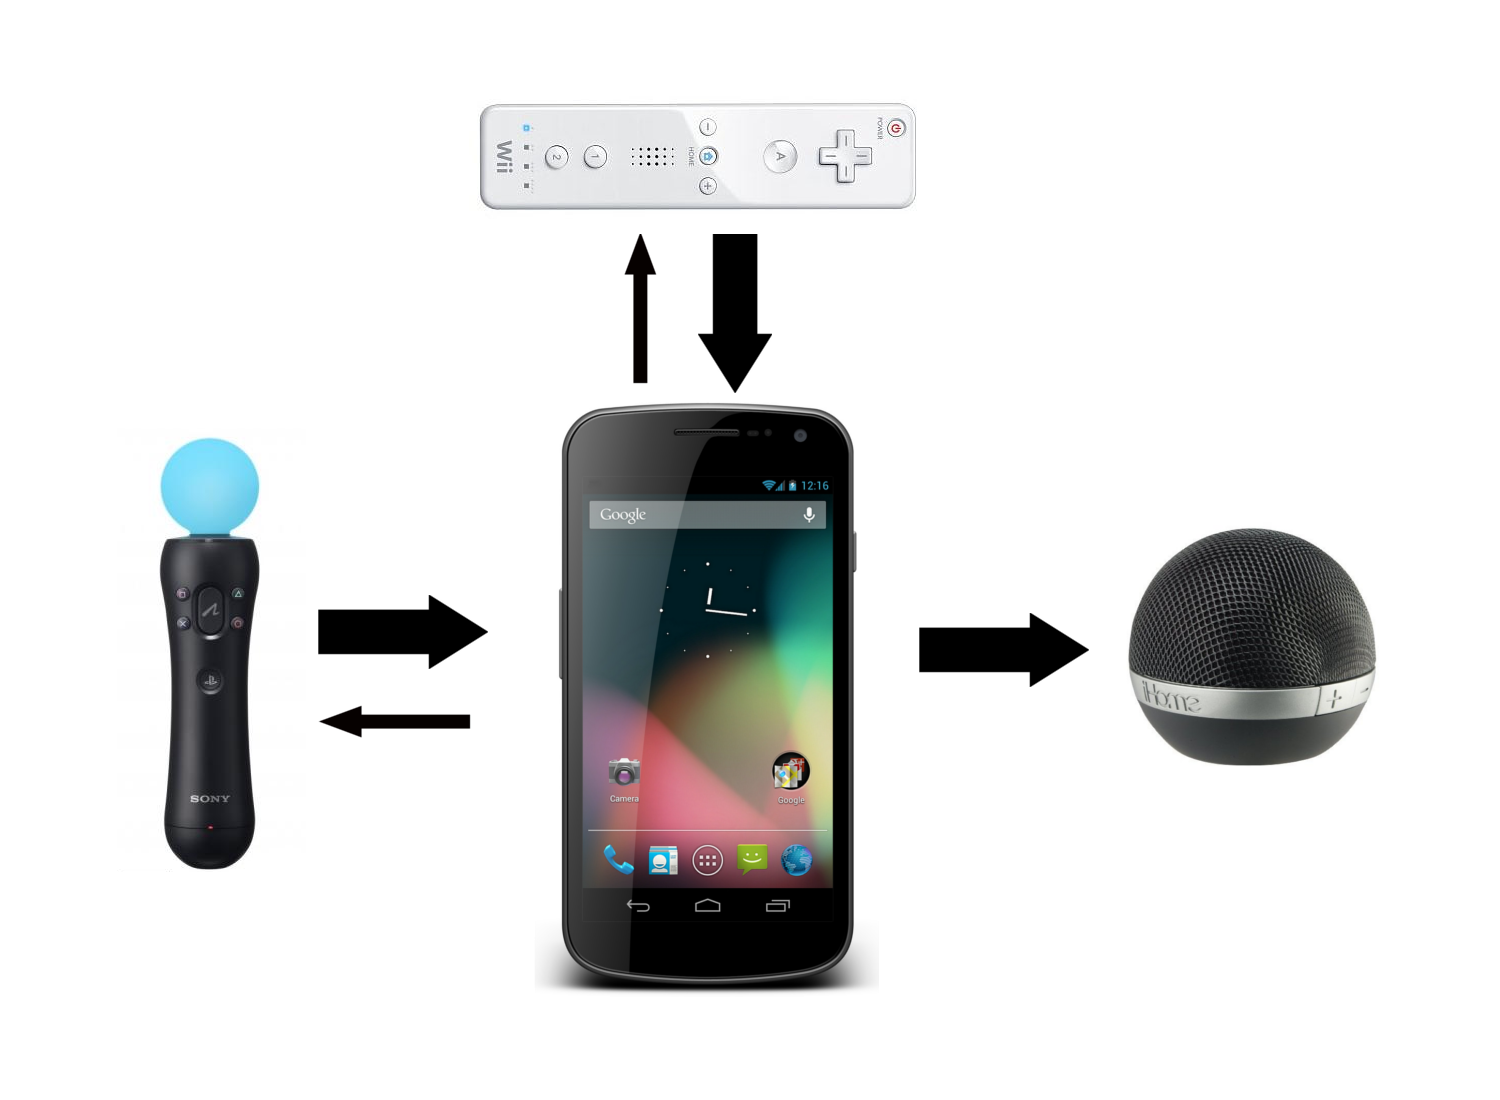
\includegraphics[width=.80\textwidth]{hub.png}
    \caption{\footnotesize A conceptual image of the hardware involved in a mobile bio-feedback system. Arrows represent the information flow, and the thickness represent the intensity.}
\end{figure}

In order to reach the primary goal mentioned above, a set of sub-goals must be completed. The sub goals will help strengthen the viability of the system in an uncontrolled changing environment.

\begin{itemize}

\item Develop a library for Android that can receive a bit stream with sensor data from a gaming peripheral via bluetooth. A Wii Remote with Motion Plus will be the first to be tested and implemented.

\item Develop a basic application that can be distributed on several Android devices. A qualitative test will be preformed in order to confirm that the application is function properly on the device.

\item Perform tests to measure the durability and of the system. Battery life, range and stability are factors that will affect the viability of the system.

\item Conduct a set of small scale tests to see if the system has any potential as a bio-feedback system.

\end{itemize}

%In this study the goal is to examine if using cheap external sensors can give more accurate and additional sensor data to help make fall detection/prevention applications more effective. The sensors examined will be the Wii Remote and the Sony Move controller. These are cheap mass produced game controllers with embedded sensors and Bluetooth support. Using Bluetooth wireless technology the sensors can be connected to the smartphone and stream supplementary acceleromter and gyroscope data.

\section{Research method}
%How the research is conducted. In the previous section you say what you are doing. Here you specify how. The choice of a research method is strictly connected to the type of questions you want to answer.
This section will provide a brief summary of the research methods that have been considered and relevant papers that present them. The final choice of research method will be presented at the end of the section, with an explanation as to why the method was chosen. Victor R. Basili\cite{paradigm} is the first paper to be looked. He identifies different experimental paradigm in Software engineering. The paper defines two main methods, the scientific method, and the mathematical method. The second paper is a guideline for conducting and reporting a case study in software engineering by Runeson and Höst.


\subsection{The Scientific Method}
The scientific method is based on observing the world, proposing a model or a theory of behaviour, measuring and analyzing and finally validating the hypothesis of the model or theory. If possible the procedure should be repeated. In software engineering this paradigm is suited when trying to understand the software process, product, people and environment. The idea is to extract some form of model that attempts to explain the underlying phenomena and evaluate whether the model is a correct representation of the phenomena being observed. An example might be when trying to understand how an organization develops software to see if a tool can be built to automate parts of the process. There are two variations of this inductive approach.

The engineering method observes existing solutions, proposes better solutions, builds the better solutions, analyzes and measure the new solution, and repeats the process until no further improvements can be made. This approach is an evolutionary improvement oriented approach which assumes one already has models of the product, software process, people and environment and focuses on modifying it in order to improve object of study. An example might be a study of tools used in the development process, and demonstrating how other tools can assist them better in their way of work then the ones they are currently using.A crucial part for this method is the need for careful analysis and measurement.

The empirical method a model is proposed, statistical/qualitative methods are developed, and applied to case studies. It results are analysed and measured, and then used to validate the model. The procedure should be repeated as to confirm findings if resources and time allow it. This paradigm is a revolutionary improvement oriented approach which begins by proposing a model that is not necessarily based upon an existing one, and atempts to study the effects of the process or product suggested by the new model. Measurment and analysis is crucial to the success of this method. Simply proposing a model or a new tool is not enough. A way to validate that the proposed model or tool is superior to the current solution must be created.

Experiments must be guided, there has to exist a rational for collecting data. The experiment must be designed to collect information suitable for building a model of the system being studied. An underlying framework must exist that will be used to interpret the collected data.

\subsection{The Mathematical Method}
The mathematical method involves proposing a formal theory or set of axioms, develop a theory, derive results and if possible compare with empirical observations. This approach is a deductive analytic model which does not require an experimental design in the statistical sense, but provides an analytic framework for developing models and understanding their boundaries based upon manipulation of the model itself. Treatment of programs as mathematical objects and their analysis of the mathematical object or its relationship to the pgroam satisfies this paradigm.

% %WRITE A GUIDELINE ABOUT CASE STUDIES HERE


There is very little to no research done on connecting smartphones and gaming peripherals together, and a working system that combines the two does not currently exist. An explorative case study will conducted in order to perform thorough research on any technical possibilities and limitations as a result of the hardware and software choices for the system. The case study seemed as a natural choice when having to create the system from scratch in the span of 3 and a half months.

The case study will be split into two parts. The first part will focus on achieving research goal (a) and (b) through a qualitative study. It will focus on the technical aspect of the goals. Technical possibilities and limitations encountered during implementation will be discussed and reported. The application will be presented in detail where architecture, functionality, and appearance of the prototype will be discussed.

The second part will focus on reaching research goal (c) and (d) through a more quantitative study. A set of tests will be outlined and conducted in order to test the durability of the system. The tests will be limited to a small amount of devices due to resource and time constraints, but several tests will be run in order to acquire reliable data.

\section{Literature review}
%This chapter provides an overview of the literature. It positions your work with respect to work already done by others
Several studies have shown that the use of biofeedback systems can reduce trunk sway \cite{multiModualBiofeedback, vibrotactileBiofeedback, vibrotactileTiltFeedback}. These studies make use of sensors strapped to test subjects in order to gather information about the position of the trunk. The sensors gathered data on the test subjects initial position, which was then processed and stored on a computer. The test subjects were then asked to challenge their balance by either walking, or standing on a balance board so that data could be collected.

\begin{figure}[h!]
  \centering
    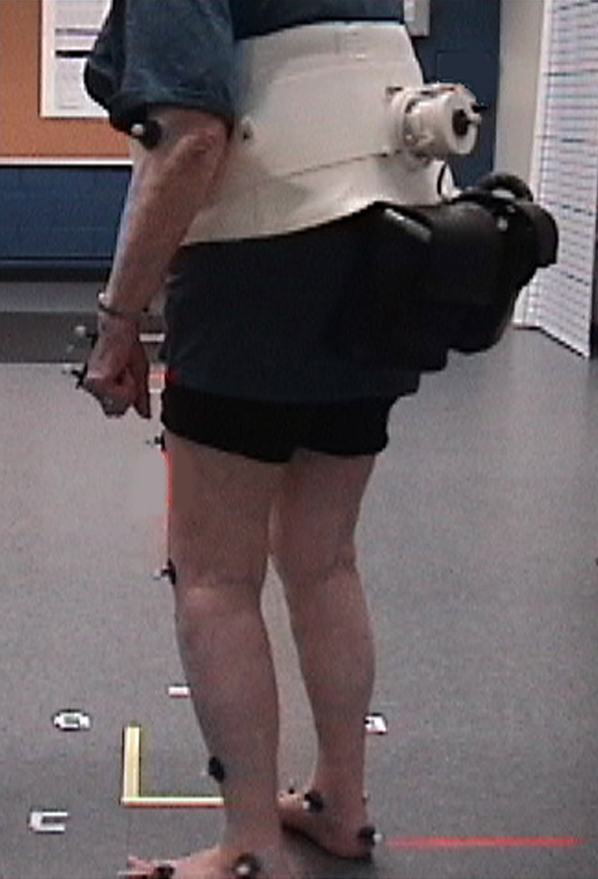
\includegraphics[width=0.40\textwidth]{sensors.png}
    \caption{\footnotesize Sensors fastened to an elderely person to detect mediolateral sway \cite{vibrotactileTiltFeedback}.}
\end{figure}

The collected data was sent to the computer in order to calculate the and compare the position of the trunk with the initial position. If trunk displacement was detected the subject was provided with feedback. The mentioned studies have primarily used vibration to give feedback about the trunk position, but light and sound was also utilized \cite{multiModualBiofeedback}.

\begin{figure}[h!]
  \centering
    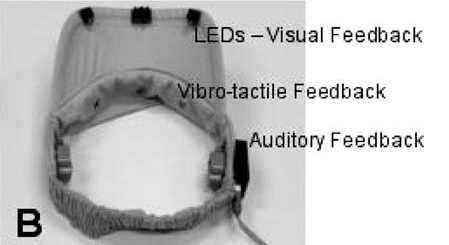
\includegraphics[width=0.80\textwidth]{biofeedback.png}
    \caption{\footnotesize Figure shows implementation of different types of biofeedback \cite{multiModualBiofeedback}.}
\end{figure}

These studies all conclude that giving vibrotactile and other types of biofeedback reduces the angular trunk displacement of patients. One of the studies showed that in some cases such systems influenced the balance of older adults \cite{multiModualBiofeedback}, while others showed improved control of mediolateral sway during gait and dynamic gait index, which are fall risk indicators in elders \cite{vibrotactileTiltFeedback}.

Making biofeedback systems available for home users creates a new set of challenges. The sensors would have to be smaller and there would be the need for a computer to interpret the information gathered by the sensors. Smartphones are one example of portable computing units with small sensors that can be used for such purposes. Several attempts have been made to create fall detection systems using smart phone technology \cite{iFall, semiSupervisedFallDetection, mobilePhoneBasedFallDetection, detectionOfFalls}, all of these studies show positive results. Sadly are no projects that focus on preventing falls through the use of smartphones and bio-feedback, all of them focus on being reacting to a fall, and not preventing it.

\subsection{iFall}
The iFall \cite{iFall} project is a lightweight Android application designed to run in the background. It monitors the data from the phones accelerometer if the accelerometer data matches a pre-defined pattern it will assume a fall has occurred. When a fall is detected the user has a certain amount of time to get up again, this is to prevent false alarms when small falls occur or the phone is dropped. If the user does not get up, a prompt window is presented that the user has to respond to, if no response is registered an alarm will be triggered. 

\begin{figure}[h!]
  \centering
    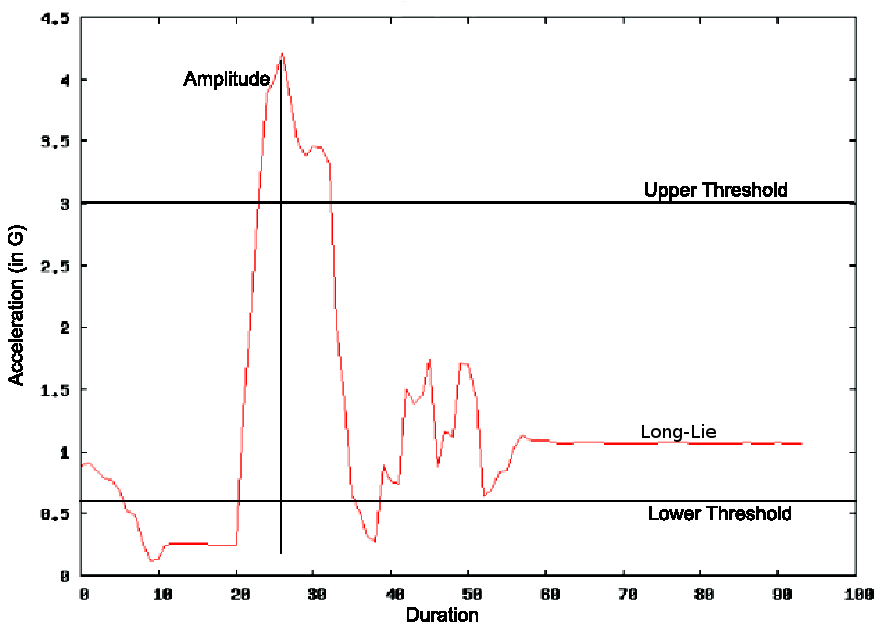
\includegraphics[width=0.80\textwidth]{patternGraph.png}
    \caption{\footnotesize An example of a classic fall. The accelerometer crossing the lower and upper amplitude  threshold followed by a long lie, recongnized this pattern as a fall.}
\end{figure}

One of the challenges the project faced was to alter and adapt the threshold depending on where the user carried the phone. Strapping it to the arm while running, or putting it inside a purse would generate more movement then on a belt clip or in a pocket. The application would identify patterns in the accelerometer data to decide where the user was most likley carrying his phone and set the appropriate thresholds. The project concludes that their software is viable and affordable, but the challenge is for the users to accept it and testing it out in the field to improve its usability.

\subsection{Placement of device}

The PerFallID\cite{fallPrevention} project and a Taiwanese Android\cite{mobilePhoneBasedFallDetection} project have similarities to the earlier iFall project, but do more research on how phone placement on the body affects the accuracy of their application. They perform a similar test by attaching the phone to Chest, Waist, and Thigh and measuring the amount of False Positive (FP) and False Negatives (FN). Strange enough they come to different conclusions when it comes to deciding the best placement for the phone; PerFallID concludes that the waist is the most accurate area, while the Taiwanese Android project concludes that the chest is the best location when using only one device with an accelerometer. The different conclusions might because different approaches and algorithms are used to detecting falls. This could mean that there is no universal optimal position for the sensors to be located.

%Figure here showing where the devices are placed

\subsection{Additional sensors}
A common limitation for the papers that have been reviews involve that only the smartphone is used as a sensors. The PerFallID implements an additional mangetic sensor that is placed above the knee. By using the data from the magnetic sensor they are able to improve the accuracy of the application, backward and lateral falls gain a significant improvement with the additional sensor. The Environmental-Adaptive Fall Detection System \cite{fallDetectionWithExtraSensors} project takes advantage of 3 sensors, and the smartphone itself acts only as a hub. The sensors are located on the waist, left ankle and right ankle. Their solution is able to detect falls with 80\% accuracy in all kinds of situations, such as running, walking, ramp, standing still, and stairs. It seems to be the biggest and most complex solution so far, which makes battery life an interesting factor, but there is no mention of it in the paper.

%Figure here showing the extra sensors system architecture?

